\hypertarget{rt__next_8c}{
\section{rt\_\-next.c File Reference}
\label{rt__next_8c}\index{rt_next.c@{rt\_\-next.c}}
}


\subsection{Detailed Description}
\begin{Desc}
\item[For internal use only.]
This file contains the implementation of the \hyperlink{group__dbprim__rbtree_ga10}{rt\_\-next()} function, used to locate the next node in a given iteration scheme.\end{Desc}


Definition in file \hyperlink{rt__next_8c-source}{rt\_\-next.c}.

{\tt \#include \char`\"{}dbprim.h\char`\"{}}\par
{\tt \#include \char`\"{}dbprim\_\-int.h\char`\"{}}\par


Include dependency graph for rt\_\-next.c:\begin{figure}[H]
\begin{center}
\leavevmode
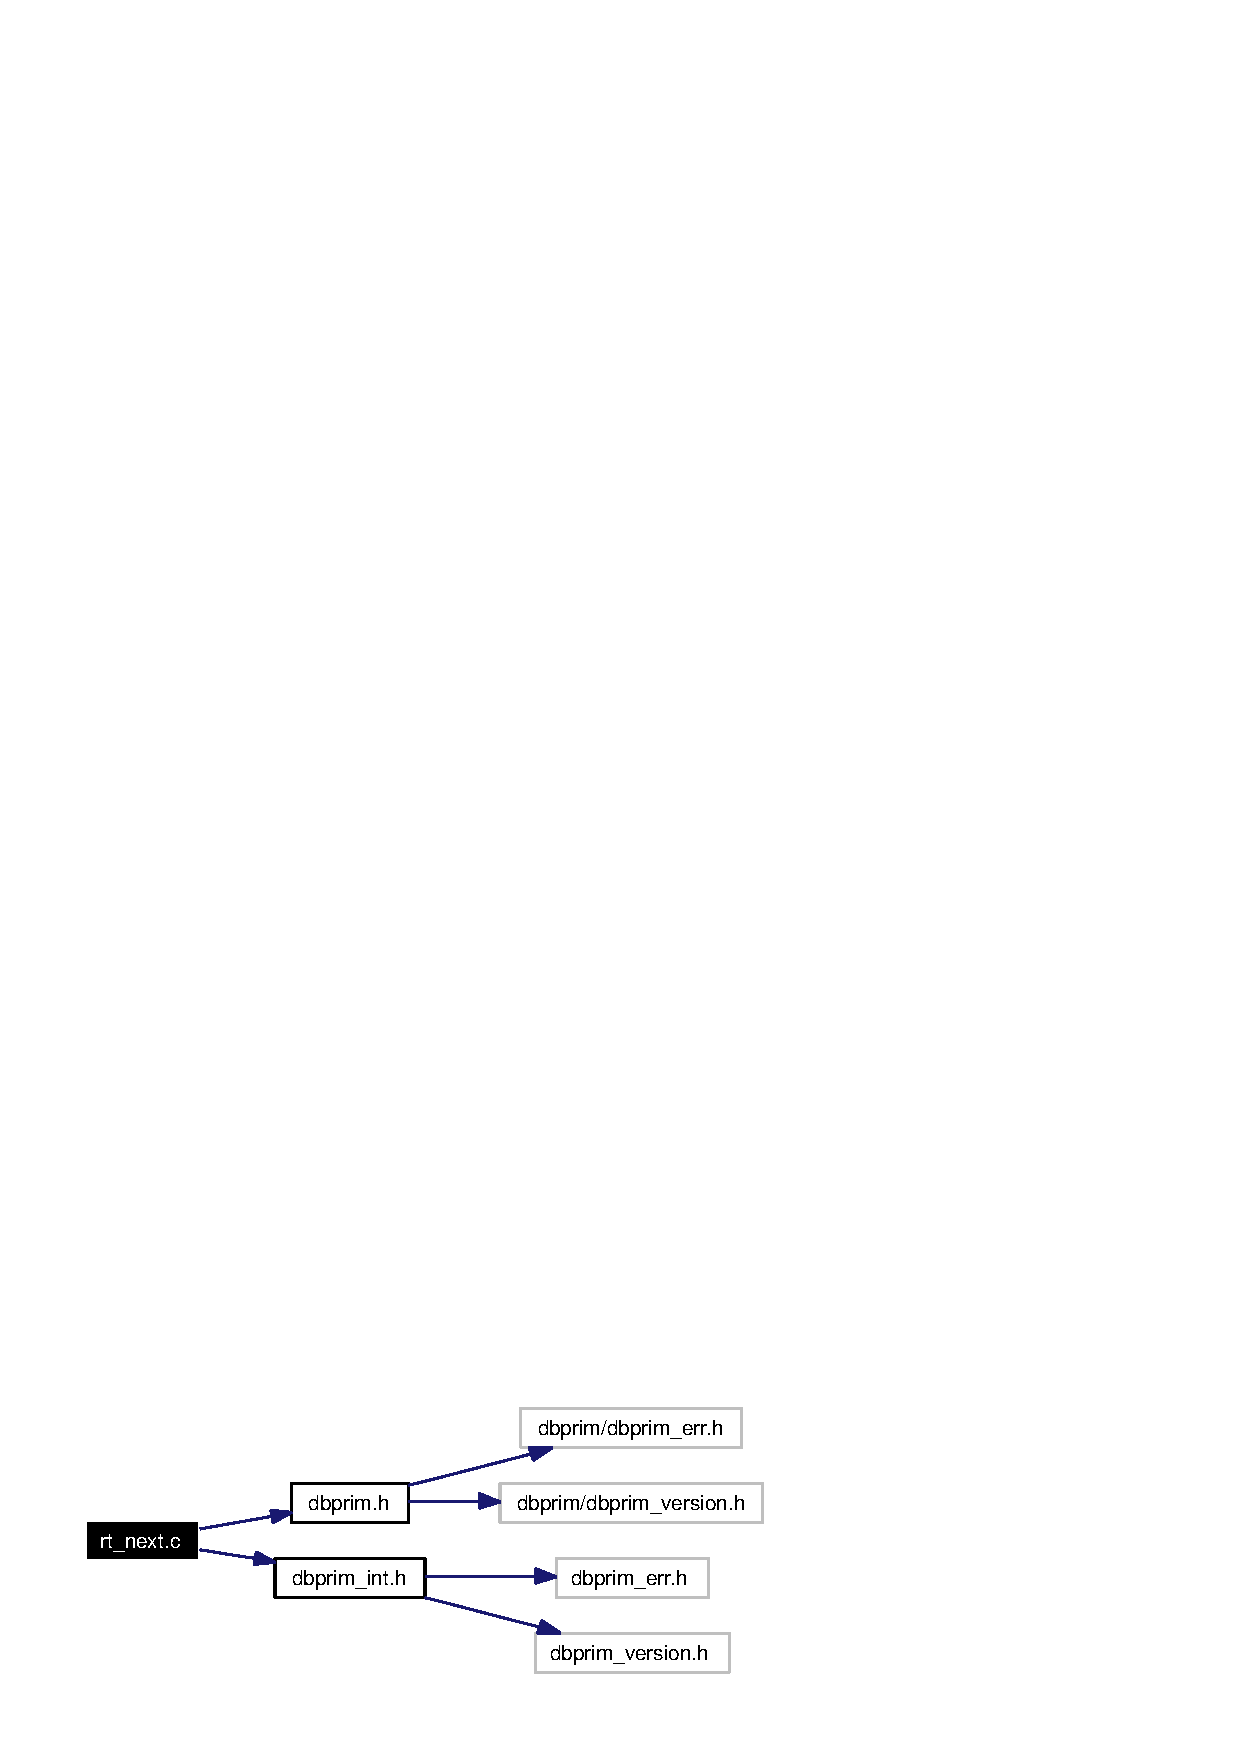
\includegraphics[width=185pt]{rt__next_8c__incl}
\end{center}
\end{figure}
\subsection*{Functions}
\begin{CompactItemize}
\item 
unsigned long \hyperlink{group__dbprim__rbtree_ga10}{rt\_\-next} (\hyperlink{struct__rb__tree__s}{rb\_\-tree\_\-t} $\ast$tree, \hyperlink{struct__rb__node__s}{rb\_\-node\_\-t} $\ast$$\ast$node\_\-io, unsigned long flags)
\begin{CompactList}\small\item\em Get the next node. \item\end{CompactList}\end{CompactItemize}
